\chapter{Software Development}
\label{chap:software-development}

\section{Software Development Methodology}
\label{section:software-development-methodology}

This project follows an iterative development methodology. Work is divided into short cycles, each focused on building and validating a specific component of the system. At the end of each cycle, the component is tested and integrated before moving to the next.

The development is organized into the following phases:

\begin{table}[H]
    \centering
    \begin{tabularx}{\textwidth}{c l X}
        \toprule
        \textbf{Phase} & \textbf{Name} & \textbf{Description} \\
        \midrule
        1 & Core AI Development & Integrate SAM 2 segmentation and tracking, SigLIP2 encoding, face matching, and rule-based deduplication for video. \\[6pt]
        2 & Backend \& Infrastructure & Set up vector database, file storage, and automated indexing pipeline with Celery task queue. \\[6pt]
        3 & Search Engine \& API & Build the REST API for search (text, image, face), hybrid scoring, and watchlist-based face matching. \\[6pt]
        4 & Web Interface \& Integration & Develop the React frontend for video upload, search, and result navigation. Full system integration. \\[6pt]
        5 & Evaluation \& Finalization & Benchmark on COCO val2017 and UCA, performance tuning, and final documentation. \\
        \bottomrule
    \end{tabularx}
    \caption{Development phases.}
    \label{tab:dev-phases}
\end{table}

\section{Technology Stack}
\label{section:technology-stack}

Table~\ref{tab:tech-stack} summarizes the technologies used in each layer of the system.

\begin{table}[H]
    \centering
    \begin{tabular}{ll}
        \toprule
        \textbf{Layer} & \textbf{Technology} \\
        \midrule
        Frontend & React, TypeScript, Tailwind CSS \\
        Backend & FastAPI (Python) \\
        Task Queue & Celery with Redis \\
        Database & PostgreSQL (pgvector) \\
        File Storage & Local filesystem / S3-compatible \\
        Segmentation & SAM 2 (Hiera) \\
        Vision-Language Encoder & SigLIP2 (ViT-B/16-256) via OpenCLIP \\
        Face Matching & InsightFace (ArcFace) \\
        Deduplication & Rule-based (frame similarity + sliding window) \\
        Deep Learning Framework & PyTorch \\
        \bottomrule
    \end{tabular}
    \caption{Technology stack.}
    \label{tab:tech-stack}
\end{table}

\section{Coding Standards}
\label{section:coding-standards}

\begin{itemize}
    \item \textbf{Python (backend and AI pipeline).} Follow PEP~8 style conventions. Use type hints for function signatures. Format code with \texttt{black} and lint with \texttt{ruff}.
    \item \textbf{TypeScript (frontend).} Follow ESLint recommended rules with Prettier formatting. Use strict TypeScript mode.
    \item \textbf{Version control.} Use Git with conventional commit messages (e.g., \texttt{feat:}, \texttt{fix:}, \texttt{refactor:}). Feature branches are merged via pull requests.
    \item \textbf{Configuration.} Sensitive values (API keys, paths) are stored in environment variables, never committed to the repository.
\end{itemize}

\section{Schedule}
\label{section:schedule}

The project spans two periods: April 2026 (pre-cooperative education) and January to March 2027 (cooperative education). The development phases listed in Table~\ref{tab:dev-phases} describe the scope of work; some phases span both periods. Figure~\ref{fig:gantt-chart} shows when each component is scheduled.

\begin{figure}[H]
    \centering
    \makebox[\textwidth]{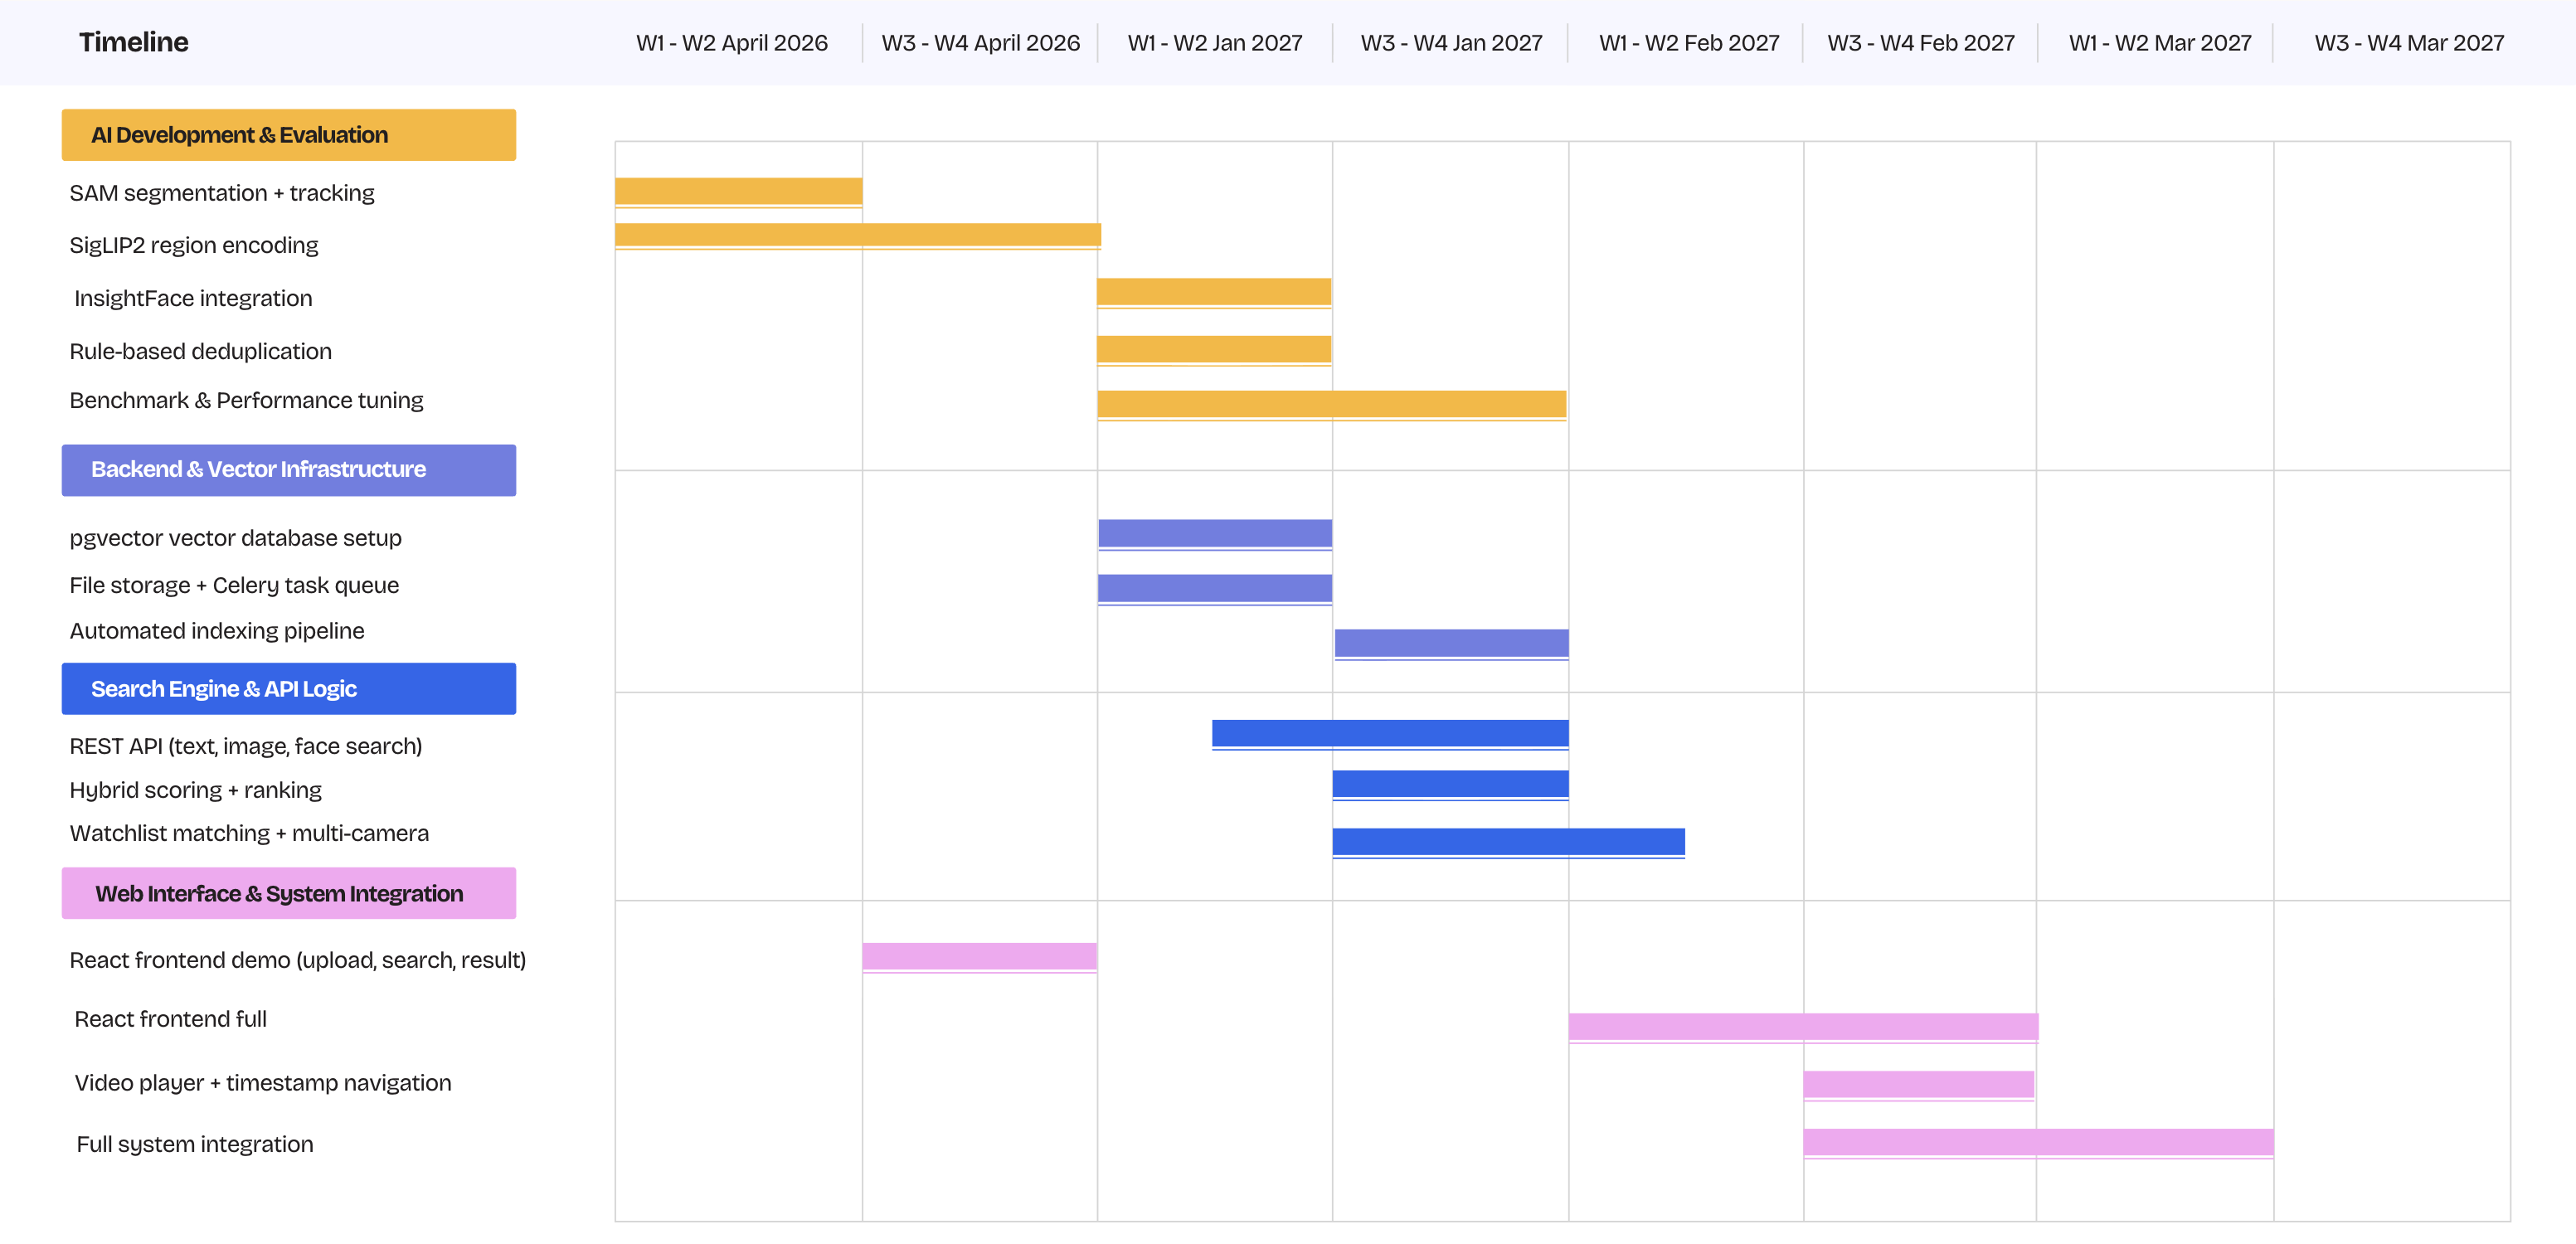
\includegraphics[width=1.2\textwidth]{assets/gantt-chart.png}}
    \caption{Project schedule (Gantt chart).}
    \label{fig:gantt-chart}
\end{figure}

The first period focuses on the core perception pipeline: integrating SAM 2 segmentation with native object tracking, SigLIP2 region encoding, and an initial React frontend demo for upload, search, and result display. The second period covers the remaining AI work (InsightFace integration, rule-based deduplication, benchmarking and performance tuning), backend infrastructure (vector database, task queue, automated indexing), search engine and API logic (hybrid scoring, watchlist-based face matching, multi-camera), and the full web interface with video player, timestamp navigation, and final system integration.

% \section{Progress Tracking Report}
% \label{section:progress-tracking-report}
% TODO: Add burndown chart or GitHub contribution graph
